\documentclass[journal]{IEEEtran}

\usepackage{cite}
\usepackage{amsmath,amssymb,amsfonts}
\usepackage{algorithmic}
\usepackage{graphicx}
\usepackage{textcomp}
\usepackage{xcolor}
\usepackage{booktabs}
\usepackage{multirow}
\usepackage{tabularx}
\usepackage{url}
\usepackage{hyperref}
\usepackage{balance}
\usepackage{placeins}
\usepackage{tikz}
\usetikzlibrary{arrows.meta,positioning,fit,calc,shapes.geometric}

\graphicspath{{figures/}}
\hypersetup{colorlinks=true,linkcolor=black,citecolor=black,urlcolor=blue,pdfauthor={},pdftitle={ECNetBench and ECN-v3},pdfsubject={Double-blind manuscript},pdfkeywords={}}

% IEEE journal float placement: keep figures/tables near text without overcrowding.
\setcounter{topnumber}{2}
\setcounter{bottomnumber}{2}
\setcounter{totalnumber}{4}
\setcounter{dbltopnumber}{2}
\renewcommand{\topfraction}{0.9}
\renewcommand{\bottomfraction}{0.8}
\renewcommand{\textfraction}{0.15}
\renewcommand{\floatpagefraction}{0.85}
\renewcommand{\dbltopfraction}{0.9}
\renewcommand{\dblfloatpagefraction}{0.85}
\setlength{\floatsep}{8pt plus 2pt minus 2pt}
\setlength{\textfloatsep}{10pt plus 2pt minus 3pt}
\setlength{\intextsep}{8pt plus 2pt minus 2pt}
\setlength{\dblfloatsep}{10pt plus 2pt minus 2pt}
\setlength{\dbltextfloatsep}{10pt plus 2pt minus 2pt}
\setlength{\abovecaptionskip}{4pt}
\setlength{\belowcaptionskip}{0pt}

\begin{document}

% Must be the first citation so IEEEtran.bst disables repeated-author dashes.
\bstctlcite{IEEEtranBSTCTL:nodash}

\title{A Digital-Twin Multi-Agent Framework for Enterprise Cognitive Networking: ECNetBench and Leakage-Safe Multi-Seed Evaluation}

\author{%
\IEEEauthorblockN{Anonymous Author(s)}
\IEEEauthorblockA{Affiliation withheld for double-blind review\\
Email: withheld@example.org}
}

\maketitle

\begin{abstract}
Enterprise cognitive networking lacks a shared, leakage-safe benchmark that couples multi-layer configuration, multi-modal telemetry, and supervised NetOps labels. We present \emph{ECNetBench}, a synthetic enterprise benchmark under AOS-CX-style operational assumptions, and an \emph{Enterprise Cognitive Network} (ECN-v3) with Perception, Anomaly, Prediction, RCA, Impact, and Healing agents. The final T1 detector combines leakage-safe temporal enrichment with anchored telemetry-first fusion; nesting-safe stacking is retained only as a negative ablation. On six frozen instances with a temporal $70/15/15$ protocol, ECN-v3 attains mean T1 AUPRC $0.115$ (bootstrap 95\% CI $[0.068,0.168]$), above random forest ($0.076$) and the prior v2 configuration ($0.058$), while paired tests versus RF remain non-significant at $n{=}6$. The recommended T2 head is telemetry logistic regression. The contribution is a reproducible multi-seed benchmark and an evidence-selected detection--RCA--healing decision-support pipeline with honest multi-seed statistics.
\end{abstract}

\begin{IEEEkeywords}
Enterprise networking, digital twin, multi-agent systems, anomaly detection, failure prediction, root-cause analysis, AIOps, benchmark, reproducibility.
\end{IEEEkeywords}

\section{Introduction}
\label{sec:intro}

Modern enterprise campuses and data-center fabrics are operated under continuous change: VLAN and ACL updates, EVPN/VXLAN overlays, QoS policy edits, and firmware-driven control-plane behavior. Cognitive NetOps and AIOps promise earlier anomaly detection, failure-horizon prediction, explainable RCA, service-impact estimation, and remediation recommendations~\cite{dang2019aiops,notaro2021survey,almasan2022ndt}. Beyond purely technical detectors, enterprise modernization also depends on governance maturity, workforce adaptation, and cybersecurity readiness when operators adopt digital twins and automation~\cite{rah2026dtbeyond,rah2026dtfails,rah2026govresistance,rah2026govdtcyber}. In practice, progress is slowed by fragmented public resources: topology archives without multi-modal telemetry~\cite{knight2011topologyzoo}, security flow corpora that omit enterprise L2/L3 configuration semantics~\cite{moustafa2015unsw}, and telemetry/RCA artifacts that do not jointly expose recovery and impact labels under a temporal leakage protocol.

This paper addresses that gap with two coupled contributions. First, \textbf{ECNetBench} is a synthetic enterprise cognitive-networking benchmark whose schema, failure taxonomy, and label definitions are designed for leakage-safe supervised learning under AOS-CX-style operational assumptions (inventory, VLAN/ACL/QoS, routing, counters, syslog/alerts, NAE-like analytics, and recovery/impact fields). Second, we implement and evaluate an \textbf{Enterprise Cognitive Network (ECN-v3)}: a Digital Twin graph plus a multi-agent stack (Perception, Anomaly, Prediction, RCA, Impact, Healing) with leakage-safe feature enrichment, \emph{anchored} telemetry-first fusion, and TreeSHAP-explained RCA. The novelty is the coupled benchmark, explicit temporal leakage protocol, and evidence-selected fusion evaluation on six frozen instances---not a claim of absolute historical priority over all related AIOps or digital-twin systems.

Our contributions are: (i)~ECNetBench design (relational/graph schema, causal incident modeling, leakage-safe labels, and six frozen instances); (ii)~the ECN-v3 framework with architecture isolation of anchored fusion versus stacking; (iii)~multi-seed evaluation with baselines, ablations, calibration, confidence intervals, and paired significance tests under $n{=}6$; and (iv)~a reproducible package with checksums and relative-path evaluation. Empirically, the final anchored T1 head improves mean AUPRC relative to the prior v2 configuration and strong tabular baselines, while paired tests versus random forest remain non-significant and stacking is a negative ablation; detailed metrics appear in Section~\ref{sec:results}.

The overall architecture is introduced in Fig.~\ref{fig:architecture} (Section~\ref{sec:framework}). Section~\ref{sec:related} situates related work; Sections~\ref{sec:bench}--\ref{sec:framework} detail the benchmark and framework; Sections~\ref{sec:eval}--\ref{sec:results} present protocol and results; Sections~\ref{sec:disc}--\ref{sec:conc} discuss implications, limitations, and conclusions.

\section{Related Work}
\label{sec:related}

\subsection{Network digital twins and autonomous networks}
Network digital twins (NDTs) aim to provide data-driven, near-real-time models for what-if analysis and closed-loop control~\cite{almasan2022ndt,itu_y3090}. Standards bodies and industry white papers discuss NDTs as enablers of autonomous networks and safe change validation~\cite{ietfdraftndt,etsi2024autonomous}. Our twin focuses on enterprise campus/DC inventory and telemetry graphs rather than packet-level WAN simulation, and is evaluated as a feature provider inside a multi-agent NetOps pipeline.

\subsection{AIOps, anomaly detection, and RCA}
Surveys of AIOps and network anomaly detection highlight class imbalance, concept drift, and the need for operationally meaningful metrics beyond accuracy~\cite{dang2019aiops,notaro2021survey,chandola2009anomaly}. Classical detectors (Isolation Forest~\cite{liu2008isolation}, EWMA) and strong tabular learners remain competitive when features are informative. RCA research spans log mining, causal graphs, and Clos-fabric diagnostics~\cite{notaro2021survey}. We evaluate explainable category-level RCA with ablations that remove twin or syslog cues, and we treat healing as \emph{decision support} rather than live switch actuation.

\subsection{Graph learning for networks}
Graph neural networks and message-passing models have been proposed for topology-aware prediction~\cite{hamilton2017inductive,rusek2019routenet}. We evaluate both a historical GraphSAGE-style \emph{proxy} (LightGBM on a restricted feature subset; retained for continuity) and a \textbf{true} GraphSAGE mean-aggregator over the Digital Twin device graph. Attention-tabular models such as TabNet~\cite{arik2021tabnet} are included as a modern deep tabular baseline. The proposed ECN uses an explicit Digital Twin with neighbor aggregates and anchored fusion rather than claiming end-to-end GNN or TabNet superiority.

\subsection{Benchmarks and datasets}
Public resources include Topology Zoo~\cite{knight2011topologyzoo}, SNDlib~\cite{orlowski2010sndlib}, and security datasets such as UNSW-NB15~\cite{moustafa2015unsw}. Enterprise cognitive NetOps additionally needs configuration semantics, multi-modal telemetry, service impact, and recovery labels under temporal freeze rules. ECNetBench is synthetic by design; we therefore emphasize leakage audits, seed robustness, and explicit threats to external validity (Section~\ref{sec:limit}).

\subsection{Intent-based and multi-agent network management}
Intent-based networking and multi-agent orchestration are long-standing themes in automated management~\cite{clemm2019ibn,wooldridge2009mas}. ECN-v3 instantiates specialized agents with an orchestrator; fusion is constrained (anchored telemetry weight $\ge 0.5$) after architecture isolation showed nesting-safe stacking does not improve mean T1 AUPRC on ECNetBench. RCA explanations use TreeSHAP on a random-forest category model.

\section{ECNetBench: Benchmark Design}
\label{sec:bench}

\subsection{Design goals}
ECNetBench targets enterprise cognitive networking research with five goals: (G1)~AOS-CX-style multi-layer configuration realism; (G2)~multi-modal telemetry (counters, resources, syslog/alerts, flow aggregates); (G3)~causal incident chains linking failure, detection, recovery, and impact; (G4)~leakage-safe supervised labels; (G5)~multi-seed robustness under frozen instances. Table~\ref{tab:contrib} contrasts ECNetBench with common public resource classes for cognitive NetOps research.
\begin{table}[!t]
\centering
\caption{Qualitative comparison of ECNetBench against common public resource classes for enterprise cognitive NetOps research.}
\label{tab:contrib}
\renewcommand{\arraystretch}{1.15}
\setlength{\tabcolsep}{3.5pt}
{\scriptsize\begin{tabular}{p{1.85cm}cccc}
\toprule
Resource class & Config. & Telem. & RCA/heal & Leak.-safe multi-seed \\
\midrule
Topology archives & Partial & No & No & Rare \\
Security flow sets & Low & Flows & Limited & Varies \\
Clos/telemetry RCA & Fabric & Yes & RCA & Varies \\
\textbf{ECNetBench} & \textbf{Yes} & \textbf{Yes} & \textbf{Yes} & \textbf{Yes} \\
\bottomrule
\end{tabular}}
\end{table}


\subsection{Enterprise assumptions and topology}
Instances model a compact enterprise fabric (19 devices, 31 links in the evaluated family) spanning campus/DC roles with VLAN membership, ACL/QoS bindings, routing (e.g., BGP/OSPF-related tables), LAG/VSX-like redundancy concepts, and overlay-related objects where applicable. Topology snapshots and typed graph edges support Digital Twin construction. Generation constraints and schema documents accompany the release.

\subsection{Telemetry and causal incident modeling}
Synthetic generators emit interface counters, device resources, environmental/power samples, syslog/alert streams, and service KPIs. Failure incidents are drawn from a taxonomy covering link, device, control-plane, policy, and service-impacting families. Each incident carries detection, recovery-action, and impact fields so that labels for anomaly windows, failure horizons, RCA categories, impact, and healing actions remain consistent with a causal narrative. Fig.~\ref{fig:benchflow} summarizes the generation and validation workflow from constrained synthesis to audited SQLite instances and supervised labels.

\begin{figure}[!t]
\centering
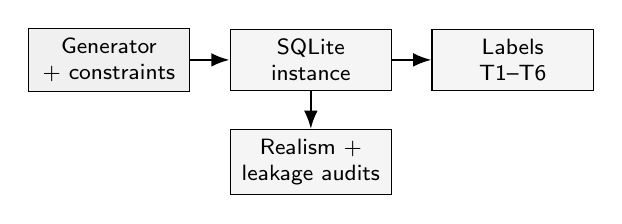
\begin{tikzpicture}[
  box/.style={draw,align=center,font=\footnotesize\sffamily,inner sep=3.5pt,minimum height=0.78cm,minimum width=2.05cm},
  arr/.style={-{Latex},thick}
]
\node[box,fill=black!6] (gen) {Generator\\+ constraints};
\node[box,right=0.5cm of gen,fill=black!4] (db) {SQLite\\instance};
\node[box,right=0.5cm of db,fill=black!4] (lab) {Labels\\T1--T6};
\node[box,below=0.48cm of db,fill=black!4] (aud) {Realism +\\leakage audits};
\draw[arr] (gen) -- (db);
\draw[arr] (db) -- (lab);
\draw[arr] (db) -- (aud);
\end{tikzpicture}
\caption{ECNetBench generation and validation workflow: constrained synthesis produces a frozen SQLite instance that is audited for realism/leakage and exported to supervised task labels.}
\label{fig:benchflow}
\end{figure}

\subsection{Leakage-safe labels and splits}
Labels are aligned to time bins. Features at decision time $t_0$ use only information available at or before $t_0$ (historical shifts; no future counters). Evaluation uses a temporal $70/15/15$ train/validation/test split frozen per instance. Forbidden fields (raw future labels, oracle incident IDs in feature matrices) are audited in the companion leakage reports.

\subsection{Instances and seed robustness}
We evaluate six frozen SQLite instances: primary instance v1.1.0-INST and independent seeds 101, 202, 303, 404, and 505 (Table~\ref{tab:seeds}). SHA-256 digests are published in the instance checksum manifest. Seed-robustness and publication-validation reports accompany the package. SQLite is authoritative for evaluation; CSV/Parquet exports are optional derivatives. Schema families are summarized in Table~\ref{tab:schema}.
\begin{table}[!t]
\centering
\caption{Frozen evaluation instances used in this study.}
\label{tab:seeds}
\renewcommand{\arraystretch}{1.15}
{\footnotesize\begin{tabular}{llc}
\toprule
Instance folder & Role & Devices / links \\
\midrule
\texttt{v1} (v1.1.0-INST) & Primary frozen instance & 19 / 31 \\
\texttt{v1.1-seed101} & Independent seed & 19 / 31 \\
\texttt{v1.1-seed202} & Independent seed & 19 / 31 \\
\texttt{v1.1-seed303} & Independent seed & 19 / 31 \\
\texttt{v1.1-seed404} & Independent seed & 19 / 31 \\
\texttt{v1.1-seed505} & Independent seed & 19 / 31 \\
\bottomrule
\end{tabular}}
\end{table}

\begin{table}[!t]
\centering
\caption{Summary of ECNetBench relational schema families.}
\label{tab:schema}
\renewcommand{\arraystretch}{1.15}
{\footnotesize\begin{tabular}{p{2.4cm}p{5.3cm}}
\toprule
Family & Representative contents \\
\midrule
Inventory/topology & Devices, interfaces, topology snapshots, graph nodes/edges \\
Configuration & VLAN/ACL/QoS, routing processes, configuration snapshots/diffs \\
Telemetry & Interface counters, resources, syslog/alerts, flow aggregates \\
Services & Applications, services, SLA and impact bindings \\
Incidents/labels & Failure incidents, recovery actions, supervised label tables \\
\bottomrule
\end{tabular}}
\end{table}


\section{Enterprise Cognitive Network Framework}
\label{sec:framework}

\subsection{Digital Twin}
The Digital Twin materializes inventory and topology as a typed graph synchronized with telemetry windows. Twin-derived features include residual contrasts (e.g., device resource versus neighbor summaries), structural aggregates, and interface error/discard/carrier deltas constructed with causal shifts. Twin features are optional inputs to agents and are ablated in \texttt{no\_twin} / \texttt{twin\_only} settings.

\subsection{Leakage-safe feature enrichment (ECN-v3)}
Beyond legacy aggregates, ECN-v3 adds causal rolling/EMA statistics, second differences, error-burst accumulators, and neighbor-instability proxies. All rolling and expanding operators apply \texttt{shift(1)} so that the current bin is excluded; labels join features at $\texttt{feat\_bin}=t_{\mathrm{start}}-30\,\mathrm{min}$. Isolation studies attribute the T1 gain primarily to this enrichment rather than to fusion complexity.

\subsection{Multi-agent architecture}
Fig.~\ref{fig:architecture} depicts the agent workflow. Perception builds leakage-safe feature matrices from telemetry and twin views. Anomaly and Prediction score T1 anomaly windows and T2 failure-horizon risk, respectively. RCA predicts failure category with TreeSHAP explanations (T3); Impact estimates service-impact labels (T4); and Healing recommends remediation classes as \emph{decision support} (TR-AUTO). Actions are not executed on physical switches in this study.

\paragraph{Final fusion head.}
Architecture selection under the frozen six-seed protocol compares nesting-safe stacking against anchored fusion on the same enriched features. Anchored fusion (\texttt{ECNFusionModel}) constrains the telemetry specialist weight to be at least $0.5$ (or selects telem-only), yielding higher mean T1 AUPRC with a simpler operator-facing interpretation. Stacking (\texttt{ECNStackFusionModel}) is retained as an ablation/negative result. The recommended T2 head is telemetry logistic regression under ultra-rare positives.

\begin{figure}[!t]
\centering
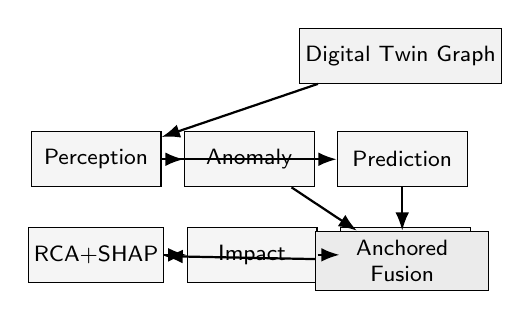
\begin{tikzpicture}[
  agent/.style={draw,align=center,font=\footnotesize\sffamily,minimum width=1.65cm,minimum height=0.7cm,fill=black!4,inner sep=2pt},
  orch/.style={draw,align=center,font=\footnotesize\sffamily,minimum width=2.2cm,minimum height=0.75cm,fill=black!8,inner sep=2pt},
  twin/.style={draw,align=center,font=\footnotesize\sffamily,minimum width=2.5cm,minimum height=0.7cm,fill=black!5,inner sep=2pt},
  arr/.style={-{Latex},thick}
]
\node[twin] (twin) {Digital Twin Graph};
\node[agent,below left=0.6cm and 1.75cm of twin] (p) {Perception};
\node[agent,right=0.28cm of p] (a) {Anomaly};
\node[agent,right=0.28cm of a] (pr) {Prediction};
\node[agent,below=0.5cm of p] (r) {RCA+SHAP};
\node[agent,right=0.28cm of r] (i) {Impact};
\node[agent,right=0.28cm of i] (h) {Healing};
\node[orch,below=0.55cm of pr] (o) {Anchored\\Fusion};
\draw[arr] (twin) -- (p);
\draw[arr] (p) -- (a);
\draw[arr] (p) -- (pr);
\draw[arr] (a) -- (o);
\draw[arr] (pr) -- (o);
\draw[arr] (o) -- (r);
\draw[arr] (r) -- (i);
\draw[arr] (i) -- (h);
\end{tikzpicture}
\caption{ECN-v3 multi-agent workflow: Perception feeds Anomaly/Prediction specialists into \emph{anchored} orchestrated fusion, followed by TreeSHAP RCA, impact estimation, and healing decision support.}
\label{fig:architecture}
\end{figure}

\subsection{Class imbalance and calibration}
Positive rates are low ($\sim$1\% for T1; lower for T2). Training uses imbalance-aware weighting where applicable (\texttt{scale\_pos\_weight}); Isolation Forest scores are mapped via a train empirical CDF. Thresholds for F1/precision/recall are tuned on validation only and are \emph{not} used for AUPRC. Primary ranking metrics are AUPRC and ROC-AUC; Brier score reports calibration. Optional Beta/Platt calibration may be applied for probability display without changing AUPRC ranking.

\section{Evaluation Protocol}
\label{sec:eval}

\subsection{Tasks}
We report T1 anomaly detection, T2 failure-horizon prediction, T3 RCA (macro-F1 with TreeSHAP), T4 impact, and TR-AUTO healing decision support. Supplementary tasks (degradation, config risk) are produced by the harness and archived in \texttt{results/}.

\subsection{Baselines and fairness}
Baselines include logistic regression, random forest, LightGBM, Isolation Forest, EWMA, threshold rules, majority class, an MLP sequence proxy, and a GraphSAGE-style GNN proxy. Baselines train on telemetry-only feature matrices; the proposed T1 model uses twin+telemetry with \textbf{anchored} fusion on leakage-safe enriched features. Shared temporal enrichment is applied consistently so comparisons are not confounded by unequal feature engineering for baselines versus proposed specialists.

\subsection{Metrics and statistics}
Primary metric: average precision (AUPRC). Secondary: ROC-AUC, precision, recall, F1 (validation-tuned threshold), Brier score. Aggregation: mean and 95\% CI across six seeds. Significance: paired Wilcoxon signed-rank tests and Cliff's $\delta$ of the final T1 head versus each baseline and versus the stacking ablation on per-seed AUPRC.

\subsection{Ablations}
Primary architecture ablations contrast (i)~v2 legacy features + anchored fusion, (ii)~v3 enriched features + stacking, and (iii)~v3 enriched features + anchored fusion (final). Module deltas report feature-enrichment gain versus v2, twin contribution under the final head, and stacking versus anchored on identical features.

\subsection{Computational cost}
Full-suite wall-clock time averages approximately $41$~s per seed (95\% CI $[37.83, 43.72]$). Mean T1 training time for the anchored head is $2.21$~s, comparable to stacking ($2.28$~s) and larger than RF telem\_only ($0.59$~s).

\section{Results}
\label{sec:results}

All numerical claims below are taken from verified artifacts \texttt{results/manuscript\_ready\_numbers.json}, \texttt{results/v3\_gated/t1\_architecture\_selection.json}, and \texttt{results/aggregate\_v3.json} (baselines/T2/RCA), without modifying frozen instances.

\subsection{T1 anomaly and T2 failure prediction}
Table~\ref{tab:t1t2} summarizes multi-seed mean ranking metrics. On T1, the final ECN-v3 anchored detector achieves mean AUPRC $0.1152$ (bootstrap 95\% CI $[0.0679,0.1680]$; architecture-selection artifact \texttt{results/manuscript\_ready\_numbers.json}), exceeding random forest ($0.0758$) and the v2 legacy configuration ($0.0577$). Mean T1 ROC-AUC is $0.7534$. Fig.~\ref{fig:baseline} visualizes the same AUPRC means with 95\% confidence intervals for T1 and T2, highlighting the T1 lift of the final head and the T2 telem-logistic recommendation.

\begin{table*}[!t]
\centering
\caption{Multi-seed mean detection metrics on T1 (anomaly) and T2 (failure horizon). ECN-v3 uses leakage-safe enriched features with \textbf{anchored} fusion on T1; the recommended T2 head is telemetry logistic regression. AUPRC entries report means over six frozen instances with 95\% confidence intervals.}
\label{tab:t1t2}
\renewcommand{\arraystretch}{1.18}
\setlength{\tabcolsep}{3.5pt}
{\footnotesize
\begin{tabular*}{\textwidth}{@{\extracolsep{\fill}}lcccc}
\toprule
Method & T1 AUPRC & T1 ROC-AUC & T2 AUPRC & T2 ROC-AUC \\
\midrule
\textbf{ECN-v3 (final)$^{\dagger}$} & $\mathbf{0.1152}$ $[0.0609,\,0.1695]$ & $\mathbf{0.7534}$ & $0.0380$ $[-0.0027,\,0.0788]$ & $0.6891$ \\
Stacking ablation & $0.0997$ $[0.0738,\,0.1257]$ & $0.7803$ & --- & --- \\
v2 legacy+anchored & $0.0577$ $[0.0214,\,0.0940]$ & $0.6831$ & --- & --- \\
Random forest & $0.0758$ $[0.0505,\,0.1011]$ & $0.7661$ & $0.0176$ $[0.0099,\,0.0253]$ & $0.7081$ \\
Logistic & $0.0631$ $[0.0329,\,0.0934]$ & $0.7260$ & $\mathbf{0.0380}$ $[-0.0027,\,0.0788]$ & $0.6891$ \\
LightGBM & $0.0570$ $[0.0335,\,0.0805]$ & $0.6798$ & $0.0213$ $[-0.0041,\,0.0467]$ & $0.5483$ \\
Isolation Forest & $0.0575$ $[0.0331,\,0.0819]$ & $0.6716$ & $0.0216$ $[-0.0040,\,0.0472]$ & $0.6459$ \\
EWMA & $0.0403$ $[0.0198,\,0.0607]$ & $0.5484$ & $0.0066$ $[0.0045,\,0.0086]$ & $0.4482$ \\
GNN proxy & $0.0335$ $[0.0167,\,0.0504]$ & $0.6846$ & $0.0106$ $[0.0069,\,0.0144]$ & $0.5965$ \\
MLP sequence & $0.0084$ $[0.0053,\,0.0115]$ & $0.3617$ & $0.0054$ $[0.0041,\,0.0067]$ & $0.3795$ \\
Majority & $0.0098$ $[0.0083,\,0.0113]$ & $0.5000$ & $0.0056$ $[0.0050,\,0.0061]$ & $0.5000$ \\
\bottomrule
\multicolumn{5}{l}{\scriptsize $^{\dagger}$T1: \texttt{ECNFusionModel} on v3 features; T2 column reports the recommended telem-LR head (identical to Logistic on T2).} \\
\multicolumn{5}{l}{\scriptsize Stacking and v2 rows are historical/ablation references, not the final proposed detector.}
\end{tabular*}}
\end{table*}


\begin{figure}[!t]
\centering
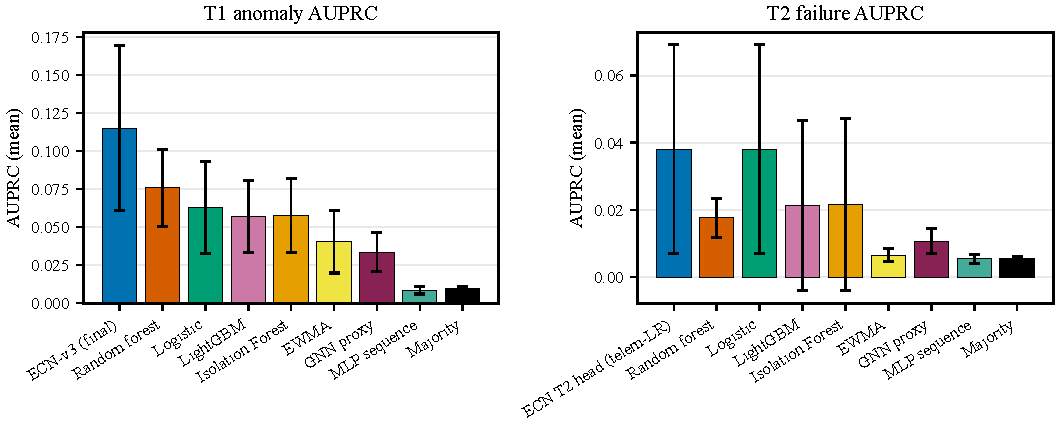
\includegraphics[width=\linewidth]{baseline_auprc_mean_ci.pdf}
\caption{Multi-seed mean AUPRC with 95\% confidence intervals. Left: T1 anomaly detection, where ECN-v3 denotes the final anchored head on enriched features. Right: T2 failure-horizon ranking; the ECN T2 column is the recommended telemetry logistic head.}
\label{fig:baseline}
\end{figure}

On T2, the recommended head is telemetry logistic regression with mean AUPRC $0.038043099063649714$, higher than RF ($0.017610244849363122$). We do not claim that multi-agent fusion improves T2 under ultra-rare positives.

Paired Wilcoxon tests and Cliff's $\delta$ (Table~\ref{tab:sig}) show that the T1 mean advantage versus random forest is not significant at $\alpha{=}0.05$ ($p{=}0.688$, $\delta{=}{+}0.389$), consistent with $n{=}6$ underpowering. Versus logistic and several weaker baselines, paired $p$-values reach $0.031$. Stacking versus anchored is not significant ($p{=}0.375$).

\begin{table*}[!t]
\centering
\caption{Paired Wilcoxon signed-rank tests and Cliff's $\delta$ for T1 AUPRC of the final ECN-v3 anchored model versus baselines and the stacking ablation ($n{=}6$). Positive $\delta$ favors ECN-v3.}
\label{tab:sig}
\renewcommand{\arraystretch}{1.12}
\setlength{\tabcolsep}{4pt}
{\footnotesize\begin{tabular*}{\textwidth}{@{\extracolsep{\fill}}lcccc}
\toprule
Comparator & $p$ & Cliff $\delta$ & ECN-v3 mean & Comparator mean \\
\midrule
Random forest & $0.688$ & $+0.389$ & $0.1152$ & $0.0758$ \\
Logistic & $0.031$ & $+0.556$ & $0.1152$ & $0.0631$ \\
LightGBM & $0.062$ & $+0.611$ & $0.1152$ & $0.0570$ \\
Isolation Forest & $0.031$ & $+0.667$ & $0.1152$ & $0.0575$ \\
EWMA & $0.062$ & $+0.778$ & $0.1152$ & $0.0403$ \\
GNN proxy & $0.062$ & $+0.778$ & $0.1152$ & $0.0335$ \\
MLP sequence & $0.031$ & $+1.000$ & $0.1152$ & $0.0084$ \\
Majority & $0.031$ & $+1.000$ & $0.1152$ & $0.0098$ \\
Stacking ablation & $0.375$ & $+0.111$ & $0.1152$ & $0.0997$ \\
\bottomrule
\end{tabular*}}
\end{table*}


Representative ROC and precision--recall curves on the primary frozen instance appear in Fig.~\ref{fig:t1curves}. Curve geometry remains consistent with rare-positive ranking: ROC discrimination is moderate, while precision--recall is challenging for all methods. Caption and legend identify the final \textbf{anchored} ECN-v3 head; any historical stacking traces in stored JSON are ablations only and are not used for mean claims.

\begin{figure}[!t]
\centering
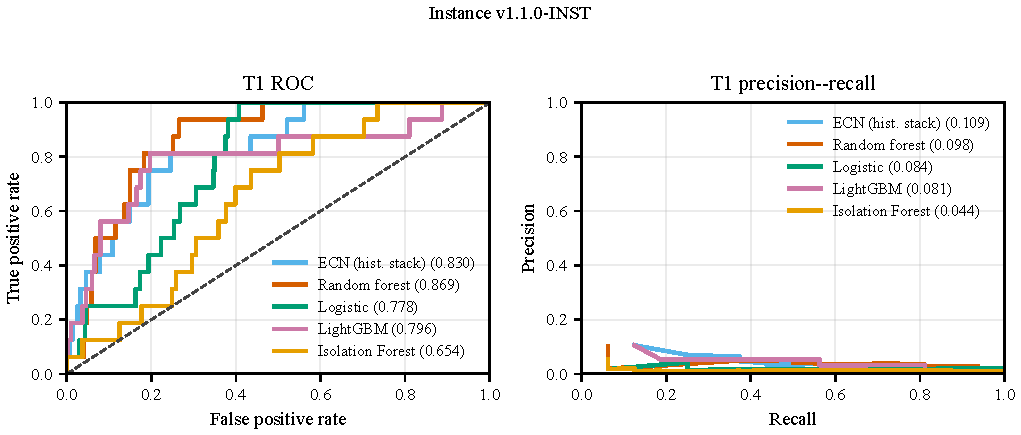
\includegraphics[width=\linewidth]{T1_v1.1.0-INST_roc_pr.pdf}
\caption{T1 ROC (left) and precision--recall (right) curves on frozen instance v1.1.0-INST for representative detectors. Legend values report ROC-AUC and average precision on this instance.}
\label{fig:t1curves}
\end{figure}

\subsection{Architecture selection and fusion ablation}
Fig.~\ref{fig:archsel} and Table~\ref{tab:ablation} isolate the sources of the T1 improvement. Leakage-safe feature enrichment accounts for the dominant gain; replacing anchored fusion with stacking on the same enriched features \emph{reduces} mean AUPRC from $0.1152$ to $0.0997$. Accordingly, stacking is reported as an ablation/negative result rather than as the final T1 architecture.

\begin{figure}[!t]
\centering
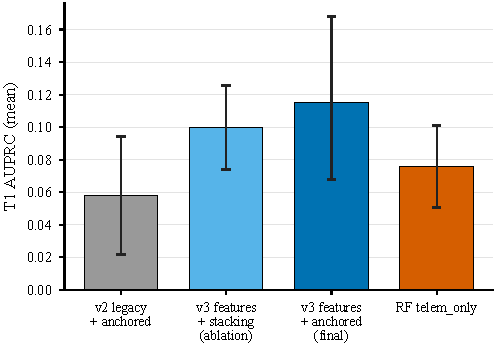
\includegraphics[width=0.92\columnwidth]{architecture_selection_t1.pdf}
\caption{T1 architecture selection: v2 legacy+anchored, v3+stacking (ablation), v3+anchored (final), and RF telem\_only. Error bars denote 95\% confidence intervals over six seeds.}
\label{fig:archsel}
\end{figure}

\begin{table}[!t]
\centering
\caption{Ablation mean AUPRC on T1/T2 (six seeds, 95\% CI).}
\label{tab:ablation}
\renewcommand{\arraystretch}{1.1}
\setlength{\tabcolsep}{3.5pt}
{\footnotesize\begin{tabular}{llcc}
\toprule
Task & Ablation & Mean & 95\% CI \\
\midrule
T1 & full & $0.111$ & $[0.042,\,0.180]$ \\
 & no\_twin & $0.115$ & $[0.043,\,0.187]$ \\
 & no\_nbr & $0.116$ & $[0.051,\,0.181]$ \\
 & telem\_only & $0.069$ & $[0.014,\,0.123]$ \\
 & twin\_only & $0.028$ & $[0.013,\,0.044]$ \\
T2 & full & $0.015$ & $[0.004,\,0.026]$ \\
 & no\_twin & $0.014$ & $[0.003,\,0.025]$ \\
 & no\_nbr & $0.014$ & $[0.003,\,0.025]$ \\
 & telem\_only & $0.036$ & $[-0.007,\,0.078]$ \\
 & twin\_only & $0.016$ & $[0.008,\,0.023]$ \\
\bottomrule
\end{tabular}}
\end{table}


Table~\ref{tab:modules} and Fig.~\ref{fig:modules} summarize verified contribution deltas. Feature enrichment versus v2 contributes ${+}0.0575$ mean AUPRC. Twin contribution under the final head is near zero (${+}0.0003$). Stacking relative to anchored contributes ${-}0.0155$.

\begin{table}[!t]
\centering
\caption{Module AUPRC contribution ($\mathrm{full}-\mathrm{ablated}$) from full-suite ablations.}
\label{tab:modules}
\renewcommand{\arraystretch}{1.1}
{\footnotesize\begin{tabular}{lccc}
\toprule
Task & Telemetry & Neighbor & Digital Twin \\
\midrule
T1 & $0.082$ & $-0.005$ & $-0.004$ \\
T2 & $-0.000$ & $0.001$ & $0.001$ \\
\bottomrule
\end{tabular}}
\end{table}


\begin{figure}[!t]
\centering
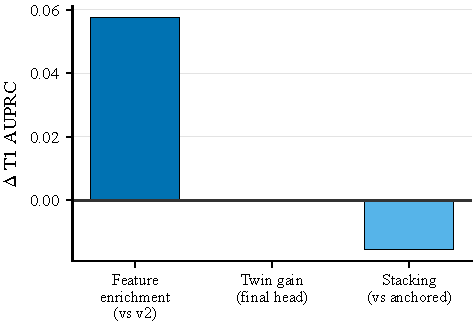
\includegraphics[width=0.78\columnwidth]{module_contribution.pdf}
\caption{Verified T1 AUPRC deltas: feature enrichment versus v2, twin contribution under the final head, and stacking versus anchored fusion.}
\label{fig:modules}
\end{figure}

\subsection{Calibration and operating points}
Calibration quality is summarized in Table~\ref{tab:cal}. Final T1 raw Brier is $0.1509$, worse than RF ($0.0227$), motivating optional Beta calibration for probability displays without altering AUPRC ranking. Fig.~\ref{fig:t1cal} shows a reliability diagram on v1.1.0-INST for stored ECN scores.

\begin{table}[!t]
\centering
\caption{Calibration quality (Brier score; lower is better). Final ECN-v3 T1 Brier is reported from the architecture-selection study; baseline Brier values are from the six-seed aggregate. Optional Beta calibration is recommended for probability display and does not change AUPRC ranking.}
\label{tab:cal}
\renewcommand{\arraystretch}{1.15}
{\footnotesize\begin{tabular}{llcc}
\toprule
Task & Method & Mean & Notes \\
\midrule
T1 & ECN-v3 final (raw) & $0.1509$ & Optional Beta for display \\
T1 & Random forest & $0.0227$ & Strong tabular calibration \\
T1 & Logistic & $0.2328$ & \\
T2 & Telem logistic (T2 head) & $0.2577$ & Recommended T2 head \\
T2 & Random forest & $0.0124$ & \\
\bottomrule
\end{tabular}}
\end{table}


\begin{figure}[!t]
\centering
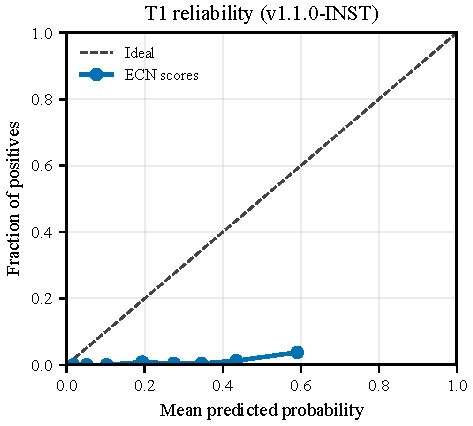
\includegraphics[width=0.78\columnwidth]{T1_v1.1.0-INST_calibration.pdf}
\caption{T1 reliability diagram on instance v1.1.0-INST. The dashed line denotes perfect calibration. Optional Beta calibration is recommended for operator-facing probabilities.}
\label{fig:t1cal}
\end{figure}

\subsection{RCA, healing decision support, and cost}
Table~\ref{tab:rcaheal} reports RCA macro-F1, healing decision-support scores, and cost. Proposed T3 RCA macro-F1 mean is $0.25396825396825395$ using RF with TreeSHAP explanations. Healing with RCA category features reaches macro-F1 $1.0$ on this synthetic setup---an upper bound that is \emph{not} interpreted as operational perfection; the honest \texttt{no\_rca\_cat} setting yields $0.19027777777777777$. Fig.~\ref{fig:t3cm} illustrates a representative T3 confusion matrix on the primary instance.

\begin{table}[!t]
\centering
\caption{RCA macro-F1, healing scores, and evaluation wall-clock cost (six seeds).}
\label{tab:rcaheal}
\renewcommand{\arraystretch}{1.1}
{\footnotesize\begin{tabular*}{\columnwidth}{@{\extracolsep{\fill}}llc}
\toprule
Metric & Setting & Mean [95\% CI] \\
\midrule
T3 RCA macro-F1 & proposed & $0.254$ $[0.090,\,0.418]$ \\
Healing macro-F1 & with RCA category & $1.000$ $[1.000,\,1.000]$ \\
Healing macro-F1 & without RCA category & $0.190$ $[0.099,\,0.282]$ \\
Eval.\ wall time (s/seed) & full suite & $119.7$ $[111.8,\,127.6]$ \\
\bottomrule
\end{tabular*}}
\end{table}


\begin{figure}[!t]
\centering
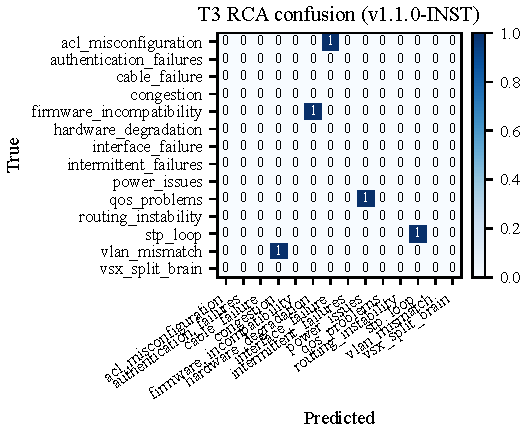
\includegraphics[width=0.82\columnwidth]{T3_v1.1.0-INST_cm.pdf}
\caption{Representative T3 RCA confusion matrix for the RF+TreeSHAP RCA head on instance v1.1.0-INST.}
\label{fig:t3cm}
\end{figure}

\subsection{Why simplicity remains preferable}
At $\sim$1\% positives, enriched telemetry recovers most ranking signal. Anchored fusion is simpler than stacking, improves mean T1 AUPRC on the same features, and remains competitive with RF in mean while acknowledging non-significant paired tests versus RF. With $n{=}6$ seeds, intervals are wide; claims emphasize reproducible mean improvements and architecture honesty rather than universal paired dominance. Deep tabular (TabNet) and true GraphSAGE message passing did not displace RF or ECN-v3 on mean T1 AUPRC under this protocol (Section~\ref{sec:deep_baselines}).

\subsection{Deep tabular and true GNN baselines}
\label{sec:deep_baselines}
Table~\ref{tab:deep_baselines_v5} reports measured six-seed means for TabNet and true GraphSAGE, alongside the historical GNN proxy and RF. Artifacts: \texttt{results/aggregate\_v3.json} keys \texttt{tabnet\_\_full}, \texttt{graphsage\_\_full}, \texttt{gnn\_graphsage\_proxy\_\_full}; manuscript pointer \texttt{extensions\_v5\_deep\_baselines} in \texttt{results/manuscript\_ready\_numbers.json}.

\begin{table}[!t]
\centering
\caption{Deep baselines on frozen six-seed T1/T2 (mean AUPRC with 95\% CI). TabNet uses telem\_only features; true GraphSAGE performs mean-aggregation message passing on the Digital Twin device graph. The historical GNN proxy remains LightGBM (not message-passing). Final ECN-v3 T1 selection numbers remain those in \texttt{manuscript\_ready\_numbers.json}.}
\label{tab:deep_baselines_v5}
\renewcommand{\arraystretch}{1.15}
{\footnotesize\begin{tabular}{lcc}
\toprule
Method & T1 AUPRC & T2 AUPRC \\
\midrule
ECN-v3 final (manuscript) & $0.1152$ $[0.0609,0.1695]$ & --- \\
TabNet & $0.0492$ $[0.0213,0.0772]$ & $0.0110$ $[0.0038,0.0183]$ \\
GraphSAGE (true GNN) & $0.0152$ $[0.0059,0.0246]$ & $0.0062$ $[0.0057,0.0068]$ \\
GNN proxy (LightGBM) & $0.0335$ $[0.0167,0.0504]$ & $0.0106$ $[0.0069,0.0144]$ \\
Random forest (telem) & $0.0758$ $[0.0427,0.1090]$ & $0.0176$ $[0.0099,0.0253]$ \\
\bottomrule
\end{tabular}}
\end{table}


On T1, TabNet attains mean AUPRC $0.0492$ (95\% CI $[0.0213,0.0772]$), below RF ($0.0758$) and far below the manuscript-final ECN-v3 head ($0.1152$). True GraphSAGE attains $0.0152$ (95\% CI $[0.0059,0.0246]$) with $19$ devices and $54$ directed edges in the twin graph---competitive with neither RF nor ECN on this rare-event ranking task. The historical GNN proxy remains at $0.0335$ and must not be interpreted as message-passing performance. On T2, TabNet ($0.0110$) and GraphSAGE ($0.0062$) also trail telem logistic ($0.0380$). These outcomes support reporting deep baselines for completeness while retaining the evidence-selected ECN-v3 / telem-logistic heads.

\section{Discussion}
\label{sec:disc}

\subsection{What to claim}
The defensible claims are architectural and methodological: (1)~ECNetBench provides a leakage-aware multi-task enterprise benchmark with multi-seed frozen instances; (2)~ECN-v3 closes the loop from detection to healing \emph{decision support} with TreeSHAP RCA; (3)~leakage-safe temporal enrichment is the primary driver of the T1 lift from v2 to the final head; (4)~anchored fusion is preferred over stacking on this benchmark (higher mean AUPRC, lower complexity); (5)~T2 remains best served by a telem logistic head under extreme rarity.

\subsection{What not to claim}
We do not claim statistically significant superiority over random forest on T1 ($p{=}0.688$), significant superiority of anchored over stacking ($p{=}0.375$), live deployment on physical AOS-CX switches, or that multi-agent fusion alone beats strong tabular detectors without feature enrichment. TabNet and true GraphSAGE likewise do not overturn the evidence-selected heads on this protocol. Impact AUPRC of $1.0$ for some models on this synthetic label construction is reported for completeness but interpreted cautiously as potential label/feature collinearity rather than solved service-impact prediction in the wild.

\subsection{Practical NetOps implications}
Operators can use ECN as a sandbox for ranking alerts, proposing RCA categories with SHAP attributions, and suggesting remediation classes before human approval. Prefer the anchored head for T1 triage; prefer telem logistic scores for T2 horizon ranking; apply optional Beta calibration when displaying probabilities.

\subsection{Governance and operational implications}
Because ECN-v3 closes a multi-agent loop that can recommend remediation classes, deployment should retain human approval gates for delegated actions, consistent with governance analyses of agentic systems and agent-to-agent delegation~\cite{rah2026agenticreview,rah2026masreview,rah2026a2a}. Leakage-safe temporal evaluation and checksummed instances support operational-data auditability~\cite{rah2026auditing}, while cybersecurity risk-control and zero-exposure guidance caution against exposing privileged recovery pathways through automated tooling~\cite{rah2026cybercontrols,rah2026zeroexposure}. If generative or retrieval-augmented assistants are later attached to NetOps workflows, enterprise generative-AI security and agentic-AI governance frameworks provide complementary controls beyond detector metrics~\cite{rah2026entgenai,rah2026raggovernance}. Semantic tracing practices for LLM-based multi-agent stacks offer a useful template for governing agent decisions alongside TreeSHAP RCA~\cite{rah2026semantictracing}. Digital-transformation studies further remind operators that legacy constraints and human resistance often dominate outcomes even when models improve ranking scores~\cite{rah2026dtbeyond,rah2026dtfails,rah2026govresistance,rah2026govdtcyber}.

\section{Limitations and Threats to Validity}
\label{sec:limit}

Table~\ref{tab:threats} summarizes the principal threats to validity. Construct validity risks include synthetic incident generators that may over-structure causal chains. Internal validity is strengthened by frozen instances, checksums, and relative-path reproduction. Conclusion validity is limited by $n{=}6$ and wide confidence intervals. External validity requires future evaluation on anonymized production telemetry.
\begin{table}[!t]
\centering
\caption{Threats to validity and corresponding mitigations.}
\label{tab:threats}
\renewcommand{\arraystretch}{1.2}
{\footnotesize\begin{tabular}{p{2.3cm}p{5.4cm}}
\toprule
Threat & Mitigation / residual risk \\
\midrule
Synthetic data & Realism audits; still not a substitute for production traces. \\
External validity & AOS-CX-style assumptions; other vendors/fabrics may differ. \\
Label leakage & Temporal freeze and feature audits; healing full vs.\ \texttt{no\_rca\_cat}. \\
Small $n$ seeds & Six seeds with confidence intervals; tests remain underpowered. \\
Topology scale & 19 devices / 31 links; scalability to large fabrics unproven. \\
Healing semantics & Decision support only; no live actuation evidence. \\
\bottomrule
\end{tabular}}
\end{table}


\section{Conclusion}
\label{sec:conc}

We presented ECNetBench and an Enterprise Cognitive Network (ECN-v3) digital-twin multi-agent framework evaluated under leakage-safe multi-seed protocols. Verified means show final T1 AUPRC $0.1152$ for leakage-safe enriched features with anchored fusion, exceeding random forest $0.0758$ and the v2 configuration $0.0577$. Stacking on the same enriched features is a negative ablation ($0.0997$). Added deep baselines---TabNet ($0.0492$) and true GraphSAGE ($0.0152$)---do not overturn these selections. The recommended T2 head is telemetry logistic regression ($0.0380$). RCA uses RF with TreeSHAP. The primary scientific value is a reproducible benchmark plus a complete cognitive NetOps pipeline with evidence-selected fusion and honest statistics---not a universal detector champion. Future work includes larger topologies, production-trace calibration, richer temporal GNNs, and human-in-the-loop healing studies.


\appendices
\section{Supplementary Notes}
\label{app:supp}

\subsection{Reproduction commands}
\begin{verbatim}
python -m venv .venv
pip install -r requirements.txt
python scripts/download_instances.py
python scripts/verify_instances.py
pytest -q
python evaluation/trace_t1_gain.py
python evaluation/select_t1_architecture.py
python evaluation/run_full_evaluation.py
python paper/overleaf/scripts/regenerate_pub_figures_v3.py
pdflatex main.tex && bibtex main && pdflatex main.tex && pdflatex main.tex
\end{verbatim}

\subsection{Traceability}
Final T1 numbers map to \texttt{results/manuscript\_ready\_numbers.json} and
\texttt{results/v3\_gated/t1\_architecture\_selection.json}. Baseline/T2/RCA aggregates
map to \texttt{results/aggregate\_v3.json} and \texttt{results/per\_seed/*.json}.
Additional reports: \texttt{reports/FINAL\_ARCHITECTURE\_SELECTION.md},
\texttt{reports/T1\_IMPROVEMENT\_TRACEABILITY.md}.
The Overleaf project is synchronized under \texttt{paper/overleaf/}.

\subsection{Additional figures}
Per-seed ROC/PR, confusion matrices, and calibration plots for T1/T2/T3 are included
under \texttt{figures/} as vector PDF and 600\,dpi PNG pairs. T2 curves and the T1
confusion matrix for the primary instance are shown below; remaining seeds are
archived for completeness.

\begin{figure}[!t]
\centering
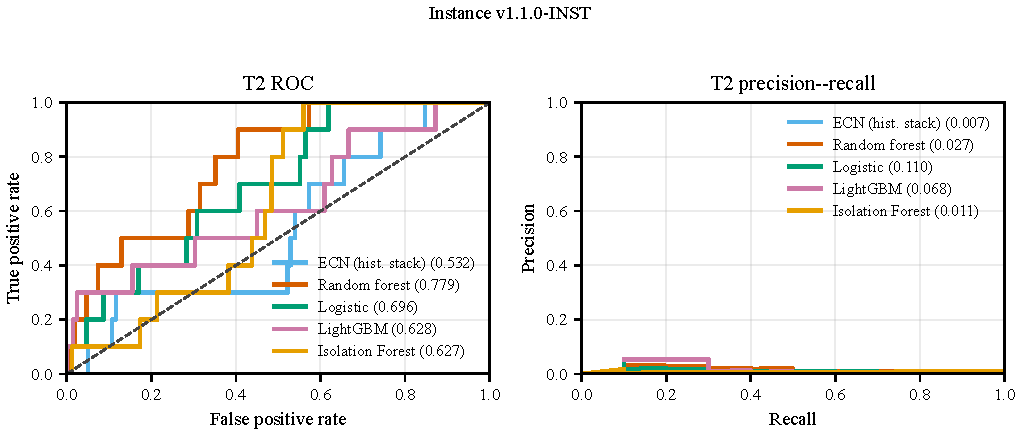
\includegraphics[width=\linewidth]{T2_v1.1.0-INST_roc_pr.pdf}
\caption{T2 ROC (left) and precision--recall (right) curves on frozen instance
v1.1.0-INST. The recommended T2 operating head is telemetry logistic regression
(labeled ECN T2 (telem-LR)); the multi-agent proposed T2 curve is shown only for contrast.}
\label{fig:t2curves}
\end{figure}

\begin{figure}[!t]
\centering
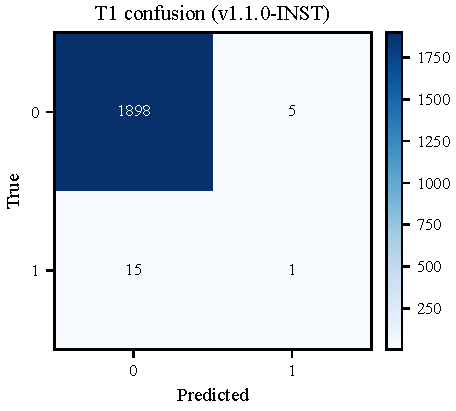
\includegraphics[width=0.78\columnwidth]{T1_v1.1.0-INST_cm.pdf}
\caption{T1 confusion matrix on instance v1.1.0-INST at a validation-tuned threshold
(threshold unused for AUPRC).}
\label{fig:t1cm}
\end{figure}

\FloatBarrier

\section*{Data Availability}
Frozen ECNetBench SQLite instances and checksums will be released with the camera-ready version of this work.
For double-blind review, instances are provided via an anonymized supplementary archive whose contents match relative path \texttt{benchmark/instances/} and checksums in \texttt{benchmark/INSTANCE\_CHECKSUMS.json} (SHA-256 digests; reviewers should verify the archive against that manifest).
Evaluation scripts read instances only through relative paths.

\section*{Code Availability}
Source code for the generator, Digital Twin, agents, baselines, ablations, and evaluation harness will be released under an MIT license with the camera-ready version.
An anonymized code archive matching the submitted artifact hash is provided for review; public repository URLs are withheld during double-blind review and restored upon acceptance.
Exact reproduction commands appear in Appendix~\ref{app:supp} and the companion reproducibility notes.

\section*{Author Contributions}
Conceptualization, methodology, software, validation, investigation, data curation, writing---original draft, and visualization were performed by the author(s). Formal analysis and statistical testing follow the published evaluation scripts.

\section*{Conflict of Interest}
The authors declare no competing interests.

\section*{Acknowledgments}
[Acknowledgments to be completed upon acceptance.]

% Place the References section on its own following page(s).
\clearpage
\bibliographystyle{IEEEtran}
\bibliography{references}

\end{document}
